\chapter{\normalsize APLIKASI}

Proses implementasi diawali dengan pengolahan data empiris berupa 
\textit{return} saham sebagai aset berisiko dan data liabilitas perusahaan 
yang diperoleh masing-masing dari harga penutupan saham dan laporan keuangan. Berdasarkan data tersebut, diturunkan 
parameter-parameter penting dalam proses optimasi portofolio seperti ekspektasi \textit{return}, matriks kovarians aset,
kovarians liabilitas, serta kovarians antara aset dan liabilitas. 
Parameter-parameter ini kemudian digunakan untuk menyusun model optimasi portofolio yang telah diturunkan sebelumnya di Bab~3, yang selanjutnya digunakan dalam penentuan bobot optimal portofolio melalui pendekatan pengali Lagrange.

\cite{Bazaraa}.



Pada bagian akhir, dilakukan analisis terhadap performa portofolio optimal yang 
dihasilkan dari model Mean-\textit{Variance} dan Mean-\textit{Value at Risk} untuk mengevaluasi pengaruh 
keberadaan liabilitas dan aset bebas risiko terhadap profil risiko dan 
\textit{return} portofolio. Hasil analisis ini memberikan pemahaman empiris 
mengenai bagaimana pertimbangan liabilitas meningkatkan relevansi model dalam 
pengelolaan portofolio pada praktik nyata \cite{Sofia}.


\section{Deskripsi Data}
Bagian ini menjelaskan data 

\begin{table}[htb]
	\caption{Definisi parameter pada model multi grup dengan intervensi pengobatan.}
	\centering
	\begin{tabular}{|c|p{6cm}|c|p{2cm}|}
		\hline
		\textbf{Parameter}& \textbf{Definisi}& \textbf{Nilai}& \textbf{Satuan}\\
		\hline
		\hline
		$A_i$ & Banyaknya individu yang lahir pada waktu-$t$ & $A_i\in [0,\infty)$ & manusia \\
		\hline
		$\beta_i$ & Laju infeksi & $\beta_i\in [0,1]$ & $\frac{1}{\text{tahun}}$ \\
		\hline
		$\mu$ & Laju kematian natural& $\mu\in [0,1]$ & $\frac{1}{\text{tahun}}$ \\
		\hline
	\end{tabular}
\label{table:32}
\end{table}

Berdasarkan penjelasan di atas, terbentuklah model penyebaran penyakit influenza di dua kota dengan intervensi pengobatan, sebagai sistem persamaan diferensial berdimensi delapan sebagai berikut.
\begin{eqnarray}\label{31}
\frac{dS_1}{dt}	&=& A_1-\frac{\beta_1 S_1(I_1+\bar{I}_2)}{S_1+I_1+\bar{S}_2+\bar{I}_2}-b_1S_1+d_1\bar{S}_1-\mu S_1+(\delta_0(1-u_1)+\delta_1u_1) I_1, \\
\frac{d\bar{I}_1}{dt}&=&b_1I_1-d_1\bar{I}_1+\frac{\beta_2 \bar{S}_1(\bar{I}_1+I_2)}{\bar{S}_1+\bar{I}_1+S_2+I_2}-(\delta_0(1-u_2)+\delta_1u_2) \bar{I}_1, \\
\frac{dS_2}{dt}&=&A_2-\frac{\beta_2 S_2(\bar{I}_1+I_2)}{S_2+I_2+\bar{S}_1+\bar{I}_1}-b_2S_2+d_2\bar{S}_2-\mu S_2+(\delta_0(1-u_2), \\
\frac{dI_2}{dt}&=&\frac{\beta_2 S_2(\bar{I}_1+I_2)}{S_2+I_2+\bar{S}_1+\bar{I}_1}-(\delta_0(1-u_2)+\delta_1u_2) I_2-b_2I_2.
\end{eqnarray}

\begin{figure}[htbp]
	\centerline{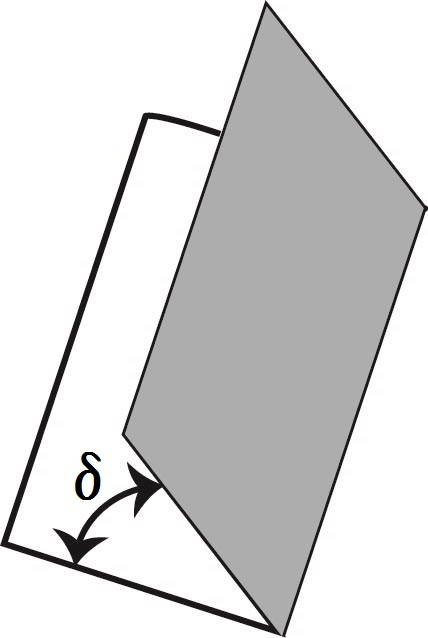
\includegraphics[scale=0.5]{gambarku/delta.jpg}}
	\caption{Sudut $\delta$} 
	\label{fig:sudut}
\end{figure}

Gambar \ref{fig:sudut} memperlihat sudut antara 2 bidang.
